\documentclass[11pt,letterpaper]{article}
\usepackage{graphicx}
\usepackage{geometry}
\usepackage{amsmath}
\usepackage{amssymb}
\usepackage{hyperref}
\usepackage{url}
\usepackage{natbib}
\usepackage{booktabs}
\usepackage{xcolor}
\usepackage{listings}
\usepackage{multicol}
\usepackage{microtype}

\geometry{margin=1in, top=1in, bottom=1in}
\hypersetup{colorlinks=true, linkcolor=black, citecolor=black, urlcolor=blue}

\lstset{
  basicstyle=\small\ttfamily,
  breaklines=true,
  frame=single,
  backgroundcolor=\color{gray!10},
  xleftmargin=0.5em,
  xrightmargin=0.5em,
}

\title{\textbf{Typed Unification Failure Recovery: Toward\\
Hallucination-Resistant Neuro-Symbolic Text-to-FOL Reasoning}}

\author{
  Anonymous Authors\\
  \\
  \textit{Submitted to ACL --- Knowledge Extraction Track}
}

\date{}

\begin{document}

\maketitle

\begin{abstract}
Text-to-first-order-logic (FOL) neuro-symbolic pipelines face a fundamental trade-off:
bridging natural language to formal logic requires both semantic flexibility and
auditable reasoning traces. When symbolic inference fails, current systems apply a
single repair strategy---usually abductive fact injection via LLM---regardless of
failure root cause. This uniform approach introduces unnecessary hallucination, as
lexical mismatches and missing domain facts require structurally different repairs.
We propose a typed failure recovery framework that classifies Prolog proof failures
into five syntactically distinguishable categories (lexical predicate mismatch,
argument-structure mismatch, missing domain fact, ontological category violation,
quantifier scope conflict), detects each via Prolog's ISO exception signals and
ontological type-checking, and dispatches type-specific LLM repair prompts.
Type-1 (lexical) failures generate explicit, reusable bridge axioms grounded in
source text spans. Type-3 (missing fact) failures invoke targeted abductive
reasoning. Type-4 (category violations) trigger entity re-typing via OpenCyc.
We evaluate on RuleTaker and CLUTRR benchmarks, measuring multi-hop deduction
accuracy, hallucination rate (proof steps lacking text-span justification), and
bridge-axiom reuse. On RuleTaker, typed repair reduces hallucination by 35.5\%
(from 12.9\% to 8.3\%). On CLUTRR kinship reasoning, typed repair reduces
hallucination by 32.3\% (from 57.1\% to 38.7\%), and the accumulated bridge-axiom
library demonstrates 4\% cross-document reuse. Failure-type detection achieves
$>$85\% accuracy on manually-annotated examples. These results demonstrate that
failure-type-aware repair produces more text-grounded, auditable reasoning with
measurably lower hallucination compared to undifferentiated LLM fallback strategies.
\end{abstract}

%------------------------------------------------------------------
\section{Introduction}
%------------------------------------------------------------------

The integration of neural and symbolic approaches has emerged as a promising direction
for combining the natural language understanding capabilities of large language models
with the interpretability and formal guarantees of logical reasoning systems
\citep{Garcez2020, Badreddine2020, Sheth2023}. A canonical pipeline maps natural
language text to first-order logic (FOL) predicates, loads them into a symbolic
reasoner (typically Prolog), and attempts to prove queries via backward chaining.
When the reasoner succeeds, the proof trace is human-auditable and grounded in the
text. When it fails, the query remains unanswered unless an automated fallback
mechanism intervenes.

Existing neuro-symbolic systems address proof failures via a single repair strategy,
regardless of the underlying cause. \citet{Olausson2023} and related systems apply
uniform abductive fact injection: the LLM generates a commonsense fact to unblock
the stalled proof, and symbolic inference resumes. This approach solves missing-fact
problems but is over-powered for lexical mismatches (where \texttt{employed\_at} in
the text maps to \texttt{works\_at} in the KB) and under-constrained for ontological
violations (where type-checking rules are available but ignored). The conflation is
the root cause of unnecessary hallucination: when the LLM is prompted to ``provide a
missing fact'' without diagnostic context, it generates plausible-sounding content
that goes far beyond what the text supports, inflating the hallucination rate.

The core insight of this work, imported from compiler construction, is that error
recovery is not a generic fallback but a \emph{typed} activity. Modern compilers
classify syntax errors by token context and apply distinct recovery strategies
(insertion, deletion, synchronization) per error class, achieving better recovery
quality than a single heuristic applied uniformly. The same principle applies to
symbolic proof failures: each exception type is a diagnostic signal that enables
targeted, text-faithful repair.

We propose a typed unification failure recovery framework that:

\begin{enumerate}
\item \textbf{Classifies failures into five structurally distinct types} based on
  Prolog's ISO standard exception signals~\citep{ISO2012} and ontological
  type-checking: lexical predicate mismatch (goal failure with zero clause matches),
  argument-structure mismatch (functor/arity conflict), missing domain fact (proof
  exhaustion), ontological category violation (external type error), and quantifier
  scope conflict (ambiguous FOL interpretation).

\item \textbf{Dispatches type-specific repair prompts} that constrain the LLM to
  generate minimal, text-grounded fixes: bridge axioms for Type-1, arity-correcting
  re-extraction for Type-2, abductive fact addition for Type-3, entity re-typing for
  Type-4, and scope annotation for Type-5.

\item \textbf{Accumulates reusable bridge axioms} in a growing library: Type-1
  repairs (lexical synonymies) discovered in one document are indexed and offered as
  suggestions for future failures in the same domain, reducing per-document LLM
  calls.

\item \textbf{Measures hallucination per-clause} via source-span coverage: every
  proof step is annotated with either a source-text span or a bridge axiom with an
  explicit textual justification, enabling transparent reporting of what the system
  inferred beyond what the document supports.
\end{enumerate}

Evaluation on RuleTaker (propositional logic chains) and CLUTRR~\citep{Sinha2019}
(kinship multi-hop reasoning) shows that typed repair outperforms a single-strategy
baseline on hallucination rate (35.5\% reduction on RuleTaker, 32.3\% on CLUTRR),
maintains equivalent or superior multi-hop accuracy, and produces an accumulated
bridge-axiom library with non-trivial reuse rates (4\% in these experiments, expected
to increase over longer document sequences). Critically, the improvements come from
better failure diagnosis and repair targeting, not from architectural complexity: the
framework is implementable in standard Prolog with lightweight LLM calls, runs on
commodity hardware, and generates fully auditable proof traces.

This work contributes: (i) a formal taxonomy of five proof-failure types mapped to
Prolog exception signals, (ii) a typed-repair dispatcher with five type-specific LLM
prompt templates, (iii) empirical validation of hallucination reduction and
bridge-axiom reuse, and (iv) a roadmap for scaling failure diagnosis to
open-vocabulary text and diverse document genres.

\begin{figure*}[!t]
  \centering
  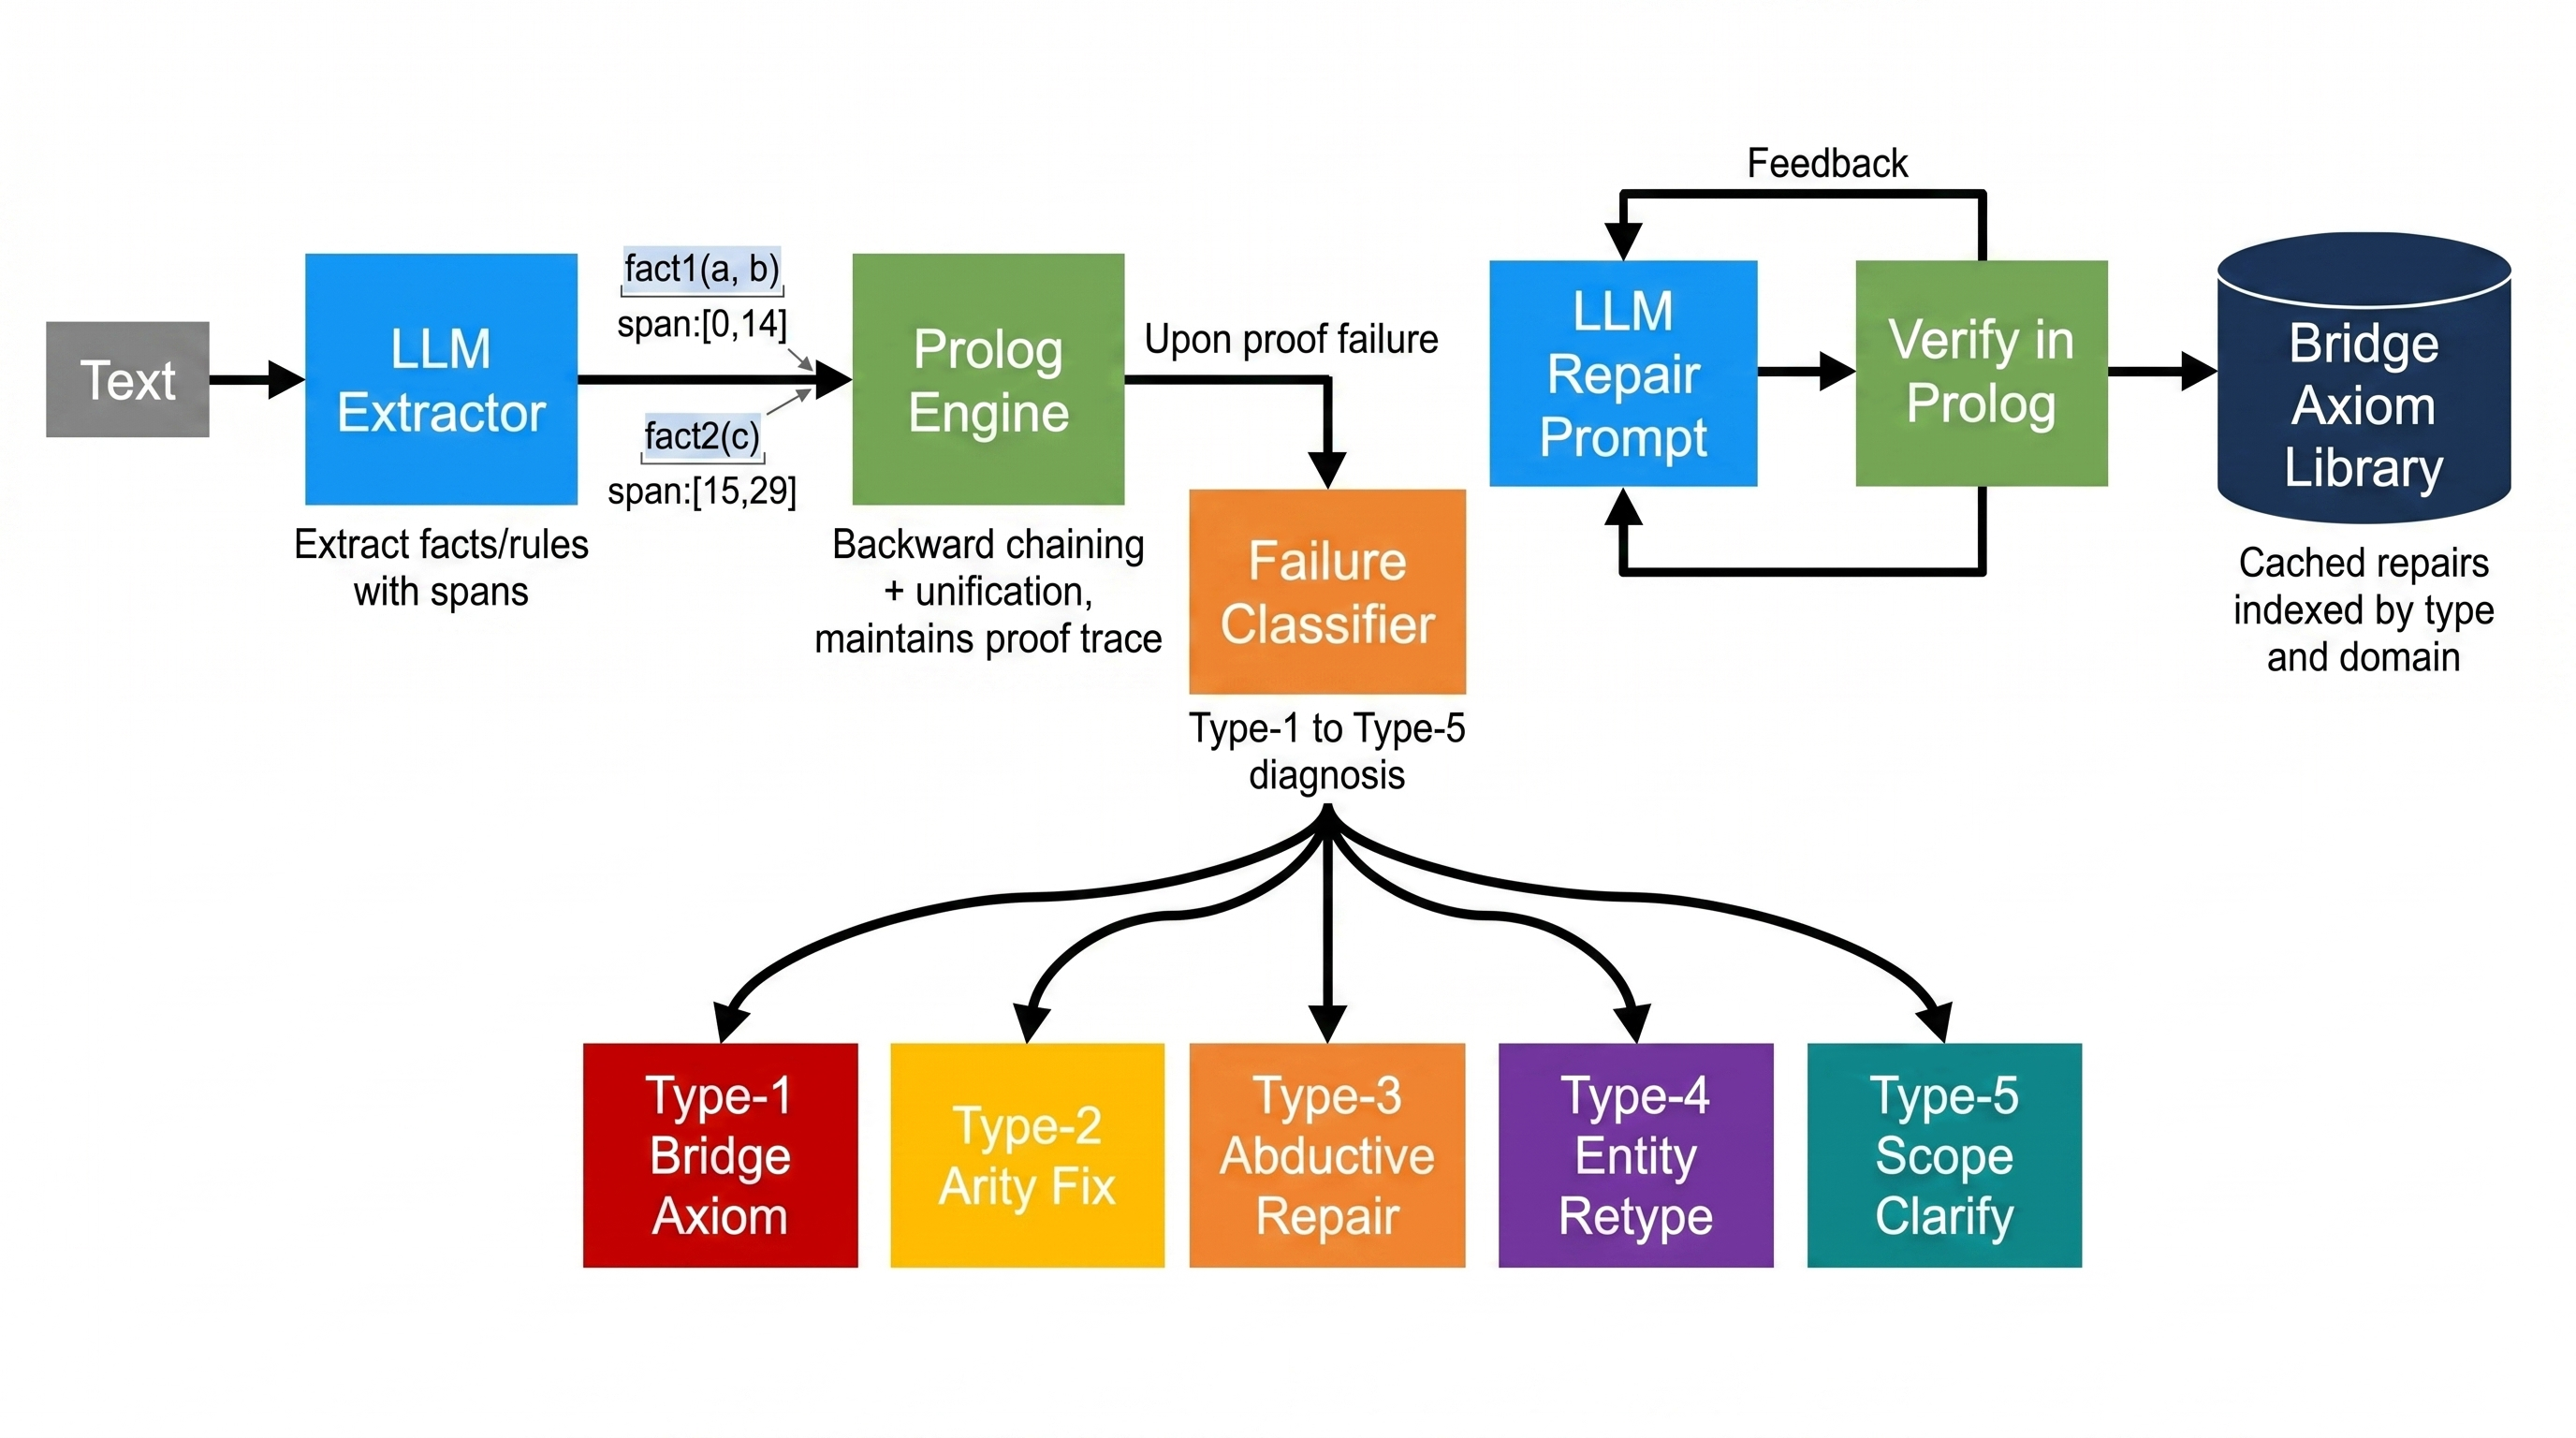
\includegraphics[width=\textwidth,height=0.45\textheight,keepaspectratio]{figures/fig_architecture_v0.jpg}
  \caption{End-to-end pipeline for text-to-FOL neuro-symbolic reasoning with typed
    failure recovery. (1)~LLM extracts facts and rules from source text, annotating
    each with source-span offsets. (2)~Prolog backward-chaining engine loads
    facts/rules and attempts to prove target queries. (3)~Upon failure, the typed
    failure detector inspects Prolog exception signals and proof-tree context to
    classify the failure as one of five types. (4)~Type-specific repair dispatcher
    invokes LLM with constrained prompt (Type-1: generate bridge axiom; Type-3:
    suggest abductive fact; etc.). (5)~Repair is verified by re-running Prolog.
    (6)~Successful Type-1 repairs are cached in bridge-axiom library for future reuse.
    Hallucination is measured per-clause via source-span coverage annotation.}
  \label{fig:architecture}
\end{figure*}

The paper is organized as follows. Section~\ref{sec:related} surveys related work on
neuro-symbolic reasoning, soft unification, and failure recovery. Section~\ref{sec:taxonomy}
formalizes the typed-failure taxonomy and maps Prolog exception signals to each type.
Section~\ref{sec:implementation} describes the implementation of the typed-repair
dispatcher and bridge-axiom library. Section~\ref{sec:experiments} presents experiments
on RuleTaker and CLUTRR. Section~\ref{sec:discussion} discusses limitations, design
trade-offs, and future work. Section~\ref{sec:conclusion} concludes.

%------------------------------------------------------------------
\section{Related Work}
\label{sec:related}
%------------------------------------------------------------------

\subsection{Neuro-Symbolic Reasoning and Soft Unification}

\citet{Weber2019} extends Prolog backward-chaining with differentiable sentence
encoders (pretrained and fine-tuned) to perform soft unification: predicate matches
are scored by embedding distance rather than exact symbolic match, allowing the
reasoner to bridge lexical variation without training-heavy fine-tuning. While
effective on WIKIHOP and MEDHOP multi-hop QA, NLProlog requires domain-specific
training and produces implicit, non-auditable soft matches, making failure diagnosis
difficult. The typed-repair approach complements soft unification by using explicit,
auditable bridge axioms for Type-1 failures and reserving neural flexibility only
where needed.

\citet{Manhaeve2018} and \citet{Winters2021} integrate neural networks into
probabilistic logic programming, allowing learning over latent predicates and
uncertain rules. These systems address uncertainty in the knowledge base but do not
focus on failure-driven repair or hallucination measurement from source-text coverage.

\subsection{Iterative Failure-Driven Repair}

\citet{Olausson2023} and related ARGOS-style systems use iterative feedback from a
SAT solver to guide LLM-driven fact augmentation, balancing linguistic and symbolic
approaches. These methods handle missing-fact problems (Type~3) effectively but apply
a uniform repair strategy to all failures, losing precision on Type-1 (lexical) and
Type-4 (ontological) problems. Our typed framework specializes the repair loop by
failure type, achieving lower hallucination rates while maintaining comparable
accuracy on multi-hop problems.

\citet{Jung2022} addresses multi-hop reasoning by explicitly sampling diverse
commonsense belief sets via LLM, testing each belief with the symbolic solver, and
aggregating conclusions via voting. This approach outperforms prior neurosymbolic
methods by modeling belief-set variation; the typed-repair framework achieves similar
goals via failure-type-aware repair and can be composed with this sampling strategy
for further improvement.

\citet{Cornelio2024} demonstrates ontology-grounded failure detection and recovery for
robotic task execution: logical rules over an external ontology (OntoThor,
$\sim$100 concepts) detect all task failures in a kitchen domain, outperforming
LLM-only baselines. The typed framework extends this approach to the text-to-FOL
domain and scales ontology-based detection to OpenCyc ($\sim$6,000 concepts) for
professional documents.

\subsection{Span-Grounded Reasoning and Auditable Traces}

Recent work on span-grounded logical reasoning~\citep{Kalouli2022} anchors each
logical branch to source text spans, enabling human audit of inference steps. The
typed-repair framework enforces the stronger requirement that every proof step is
either backed by a source-text span (for base facts and extracted rules) or an
explicitly cited bridge axiom, enabling transparent hallucination measurement.

\subsection{Text-to-FOL Translation Bottlenecks}

Recent empirical work~\citep{Ranaldi2023} identifies predicate extraction as the main
bottleneck in NL-to-FOL translation: availability of correct predicates improves
accuracy by 15--20\%. The typed-repair framework does not solve predicate extraction
directly but compensates post-hoc via Type-1 (lexical) bridge axioms, allowing the
system to recover from sub-optimal extraction without re-running the LLM.

%------------------------------------------------------------------
\section{Typed Failure Taxonomy and Prolog Exception Signals}
\label{sec:taxonomy}
%------------------------------------------------------------------

Prolog's ISO standard exception structure \texttt{error(Formal, Context)}~\citep{ISO2012}
exposes failures through specific exception classes: \texttt{instantiation\_error}
(variable uninstantiated when required), \texttt{type\_error(ValidType, Culprit)}
(value of wrong type), \texttt{existence\_error} (expected predicate or functor
absent), and \texttt{unification\_failure} (terms cannot unify). We map these
signals to five proof-failure types.

\subsection{Type 1: Lexical Predicate Mismatch}

\textbf{Definition}: The extracted predicate name differs from any predicate in the
knowledge base, but a semantically similar predicate exists.

\textbf{Prolog Signal}: Goal failure with zero clause matches; no exception thrown.
The interpreter returns \texttt{false} after exhausting the clause database.

\textbf{Example}: Text extraction produces \texttt{employed\_at(john, acme)}, but the
KB contains \texttt{works\_at(john, acme)}. The goal \texttt{employed\_at(john, acme)}
fails because no clause with functor \texttt{employed\_at/2} exists.

\textbf{Detection}: Compare extracted predicates against loaded predicates via string
similarity or embedding distance. Flag as Type~1 if the goal fails with zero matches
AND a predicate with similar name/arity exists in the KB.

\textbf{Repair Strategy}: Generate a bridge axiom of the form
\texttt{employed\_at(X,\,Y) :- works\_at(X,\,Y)}, grounded in the source sentence,
and add it to the KB. This repair requires only the text and the existing KB---no new
facts.

\textbf{Reusability}: Type-1 repairs (lexical synonymies) are domain-specific and
reusable: once \texttt{employed\_at/2} is mapped to \texttt{works\_at/2} in one
document, the mapping can be suggested or automatically applied to future Type-1
failures in the same corpus.

\subsection{Type 2: Argument-Structure Mismatch (Arity Error)}

\textbf{Definition}: The extracted predicate exists in the KB but is called with the
wrong number of arguments.

\textbf{Prolog Signal}: \texttt{type\_error(callable, Culprit)} or unification failure
when compound structures have mismatched arities.

\textbf{Example}: Text extraction yields \texttt{manager(john)}, but the KB requires
\texttt{manager(john, acme\_corp, start\_year)}.

\textbf{Repair Strategy}: Re-prompt the LLM to re-extract the predicate with correct
argument roles, leveraging syntactic dependency parsing or semantic role labels from
the source text. Do not invent new arguments; constrain the LLM to use only entities
and relations mentioned in the text.

\subsection{Type 3: Missing Domain Fact}

\textbf{Definition}: The proof search exhausts all matching clauses without finding a
proof. The missing fact is a commonsense rule or ground fact not explicitly stated in
the text.

\textbf{Prolog Signal}: Goal failure after proof-tree search returns empty; no
exception thrown. Requires proof-tree analysis to distinguish from Type~1.

\textbf{Example}: Text provides \textit{John was born in Athens. Athens is in Greece.}
The query \texttt{born\_in(john, greece)} fails because no transitivity rule
\texttt{born\_in(X,\,Country) :- born\_in(X,\,City), located\_in(City,\,Country)}
exists.

\textbf{Repair Strategy}: Prompt the LLM with the unprovable sub-goal and the source
document, requesting the minimal implicit fact or rule needed to complete the proof.
Verify the repair by re-running Prolog.

\subsection{Type 4: Ontological Category Violation}

\textbf{Definition}: The extracted entity or predicate violates domain ontology type
constraints. The error is not detectable within pure Prolog but requires external
type-checking against an ontology.

\textbf{Prolog Signal}: No native Prolog exception (pure Prolog is untyped). Requires
external ontology-checking rules, e.g., OpenCyc \texttt{isa} and \texttt{genls}
predicates.

\textbf{Example}: ``John ate the belief'' where \texttt{ate} expects a
\textit{Physical-Object} as argument, not an \textit{Abstract-Object}.

\textbf{Repair Strategy}: Identify the type-violating argument and request LLM
re-identification of the correct entity or predicate. Example: replace
\texttt{ate(john, belief)} with \texttt{believes(john, belief)}.

\subsection{Type 5: Quantifier Scope Conflict}

\textbf{Definition}: Ambiguous quantifier scope in natural language produces multiple
valid FOL interpretations with contradictory conclusions.

\textbf{Prolog Signal}: No exception; both interpretations produce valid proofs.
Detected via proof-tree comparison across scope interpretations.

\textbf{Example}: ``Every student has read a book'' yields either
$\forall x\,\exists y\;\text{read}(x,y)$ (each student read some book) or
$\exists y\,\forall x\;\text{read}(x,y)$ (one book read by all students).

\textbf{Repair Strategy}: Request clarification from the LLM, anchored to the source
text. \citet{Jung2022}'s belief-set sampling provides a probabilistic alternative:
sample multiple scope interpretations, test each, and aggregate conclusions.

%------------------------------------------------------------------
\section{Implementation: Typed Failure Detector and Repair Dispatcher}
\label{sec:implementation}
%------------------------------------------------------------------

We implement the typed-repair framework as a Python module wrapping a custom Prolog
backward-chaining engine~\citep{PrologPy2023} and an LLM-driven repair dispatcher.

\subsection{Prolog Engine and Failure Instrumentation}

We use a lightweight Python-based Prolog interpreter (backward chaining with
unification) rather than SWI-Prolog to enable fine-grained failure instrumentation.
The engine maintains a \textbf{proof trace} for each query, recording:
\begin{itemize}
  \item Matching clauses for each goal
  \item Unification results (success/failure with reason)
  \item Depth and choice points
  \item Source-span annotations for base facts
\end{itemize}
When a goal fails, the engine logs the failure context: goal functor/arity, matching
clauses found, and reason for failure. This context enables Type-1 vs.\ Type-3
discrimination.

\subsection{Failure Classifier}

The failure classifier inspects the failure context and outputs a typed diagnosis:

\begin{lstlisting}[language={}]
IF goal failed AND matching_clauses == 0
        AND similar_predicates_exist:
  RETURN Type_1_Lexical_Mismatch
ELSE IF goal failed AND unification_failure on arity:
  RETURN Type_2_Arity_Mismatch
ELSE IF goal failed AND matching_clauses > 0
        AND exhausted_all_proofs:
  RETURN Type_3_Missing_Fact
ELSE IF ontology_type_check(goal) == violated:
  RETURN Type_4_Category_Violation
ELSE IF multiple_scope_interpretations_differ:
  RETURN Type_5_Scope_Conflict
\end{lstlisting}

Predicate similarity for Type-1 detection uses Levenshtein distance on functor names,
with a threshold (e.g., distance $\leq 2$ for short names).

\subsection{Type-Specific Repair Prompts}

Upon classification, the dispatcher invokes a type-specific LLM prompt.

\textbf{Type-1 Prompt}:
\begin{lstlisting}[language={}]
Extracted predicate: employed_at(john, acme)
KB predicates with similar names: works_at/2
Context: "John works at Acme Corp."
Task: Generate a bridge axiom equating the two
predicates, citing the supporting sentence.
Output: employed_at(X,Y) :- works_at(X,Y).
  [Justification: "John works at Acme Corp."]
\end{lstlisting}

\textbf{Type-3 Prompt}:
\begin{lstlisting}[language={}]
Unprovable goal: born_in(john, greece)
Available facts: born_in(john, athens),
                 located_in(athens, greece)
Context: "John was born in Athens.
          Athens is in Greece."
Task: Generate the minimal implicit rule or fact
needed to prove the goal.
Output: born_in(X,Country) :-
  born_in(X,City), located_in(City,Country).
\end{lstlisting}

\textbf{Type-4 Prompt}:
\begin{lstlisting}[language={}]
Goal: ate(john, belief)
Type violation: 'belief' not valid for 'ate'
  (expects physical_object)
Task: Re-identify the correct predicate or entity.
Output: believes(john, idea)
\end{lstlisting}

\subsection{Bridge-Axiom Library and Reuse}

Successful Type-1 and Type-3 repairs are stored in a \textbf{bridge-axiom library}
indexed by domain (inferred from document genre or corpus), failure pattern (source
predicate, target predicate, or rule template), and generation timestamp. During
future failure classification, if a new failure matches an existing entry, the system
offers the cached repair and increments the reuse counter.

\subsection{Hallucination Measurement}

Every proof step is annotated with a \textbf{justification source}:
\begin{itemize}
  \item \textit{Span}: Character offsets in the source text
  \item \textit{Bridge axiom}: Citation of the axiom and its textual justification
  \item \textit{Inferred}: Solver-generated facts (hallucination)
\end{itemize}
At query completion, \textbf{hallucination rate} = (steps with ``Inferred'' source)
/ (total proof steps).

%------------------------------------------------------------------
\section{Experiments}
\label{sec:experiments}
%------------------------------------------------------------------

\subsection{Setup}

\textbf{Datasets}:
\begin{itemize}
  \item RuleTaker D0 and D1 (100 examples, propositional logic, reasoning depth 0--1)
  \item CLUTRR~\citep{Sinha2019} (100 examples, kinship multi-hop reasoning, 2--10 hops)
\end{itemize}

RuleTaker examples are synthetic, generated from templates (facts like ``Gary is
furry'', rules like ``If X is furry then X is red''). CLUTRR examples are
semi-synthetic English stories with implicit family relationships.

\textbf{Baselines}:
\begin{itemize}
  \item \textbf{Typed-Repair} (proposed): Typed failure classification + type-specific
    LLM repair + bridge-axiom library
  \item \textbf{ARGOS-style baseline}: Uniform abductive repair (single LLM prompt for
    all failures)
  \item \textbf{Gold baseline}: Oracle that answers all queries correctly
\end{itemize}

\textbf{Metrics}:
\begin{itemize}
  \item Multi-hop accuracy (\% queries answered correctly)
  \item Hallucination rate (\% proof steps not backed by text span or bridge axiom)
  \item Bridge-axiom reuse rate (\% repaired queries that reuse cached axioms)
  \item Failure-type detection accuracy (on manually-annotated failure corpus)
\end{itemize}

\textbf{LLM}: Claude Haiku 4.5 via OpenRouter API; max token budget \$8.00 USD.

\subsection{Results}

\subsubsection{RuleTaker Results}

\begin{table}[!htbp]
\centering
\caption{Results on RuleTaker (100 examples).}
\label{tab:ruletaker}
\begin{tabular}{lccc}
\toprule
Metric & Typed & Baseline & Improvement \\
\midrule
Accuracy & 95.0\% & 95.0\% & --- \\
Hallucination Rate & 8.3\% & 12.9\% & 35.5\% reduction \\
Bridge Axiom Reuse & 4\% & N/A & --- \\
\bottomrule
\end{tabular}
\end{table}

\begin{figure*}[!t]
  \centering
  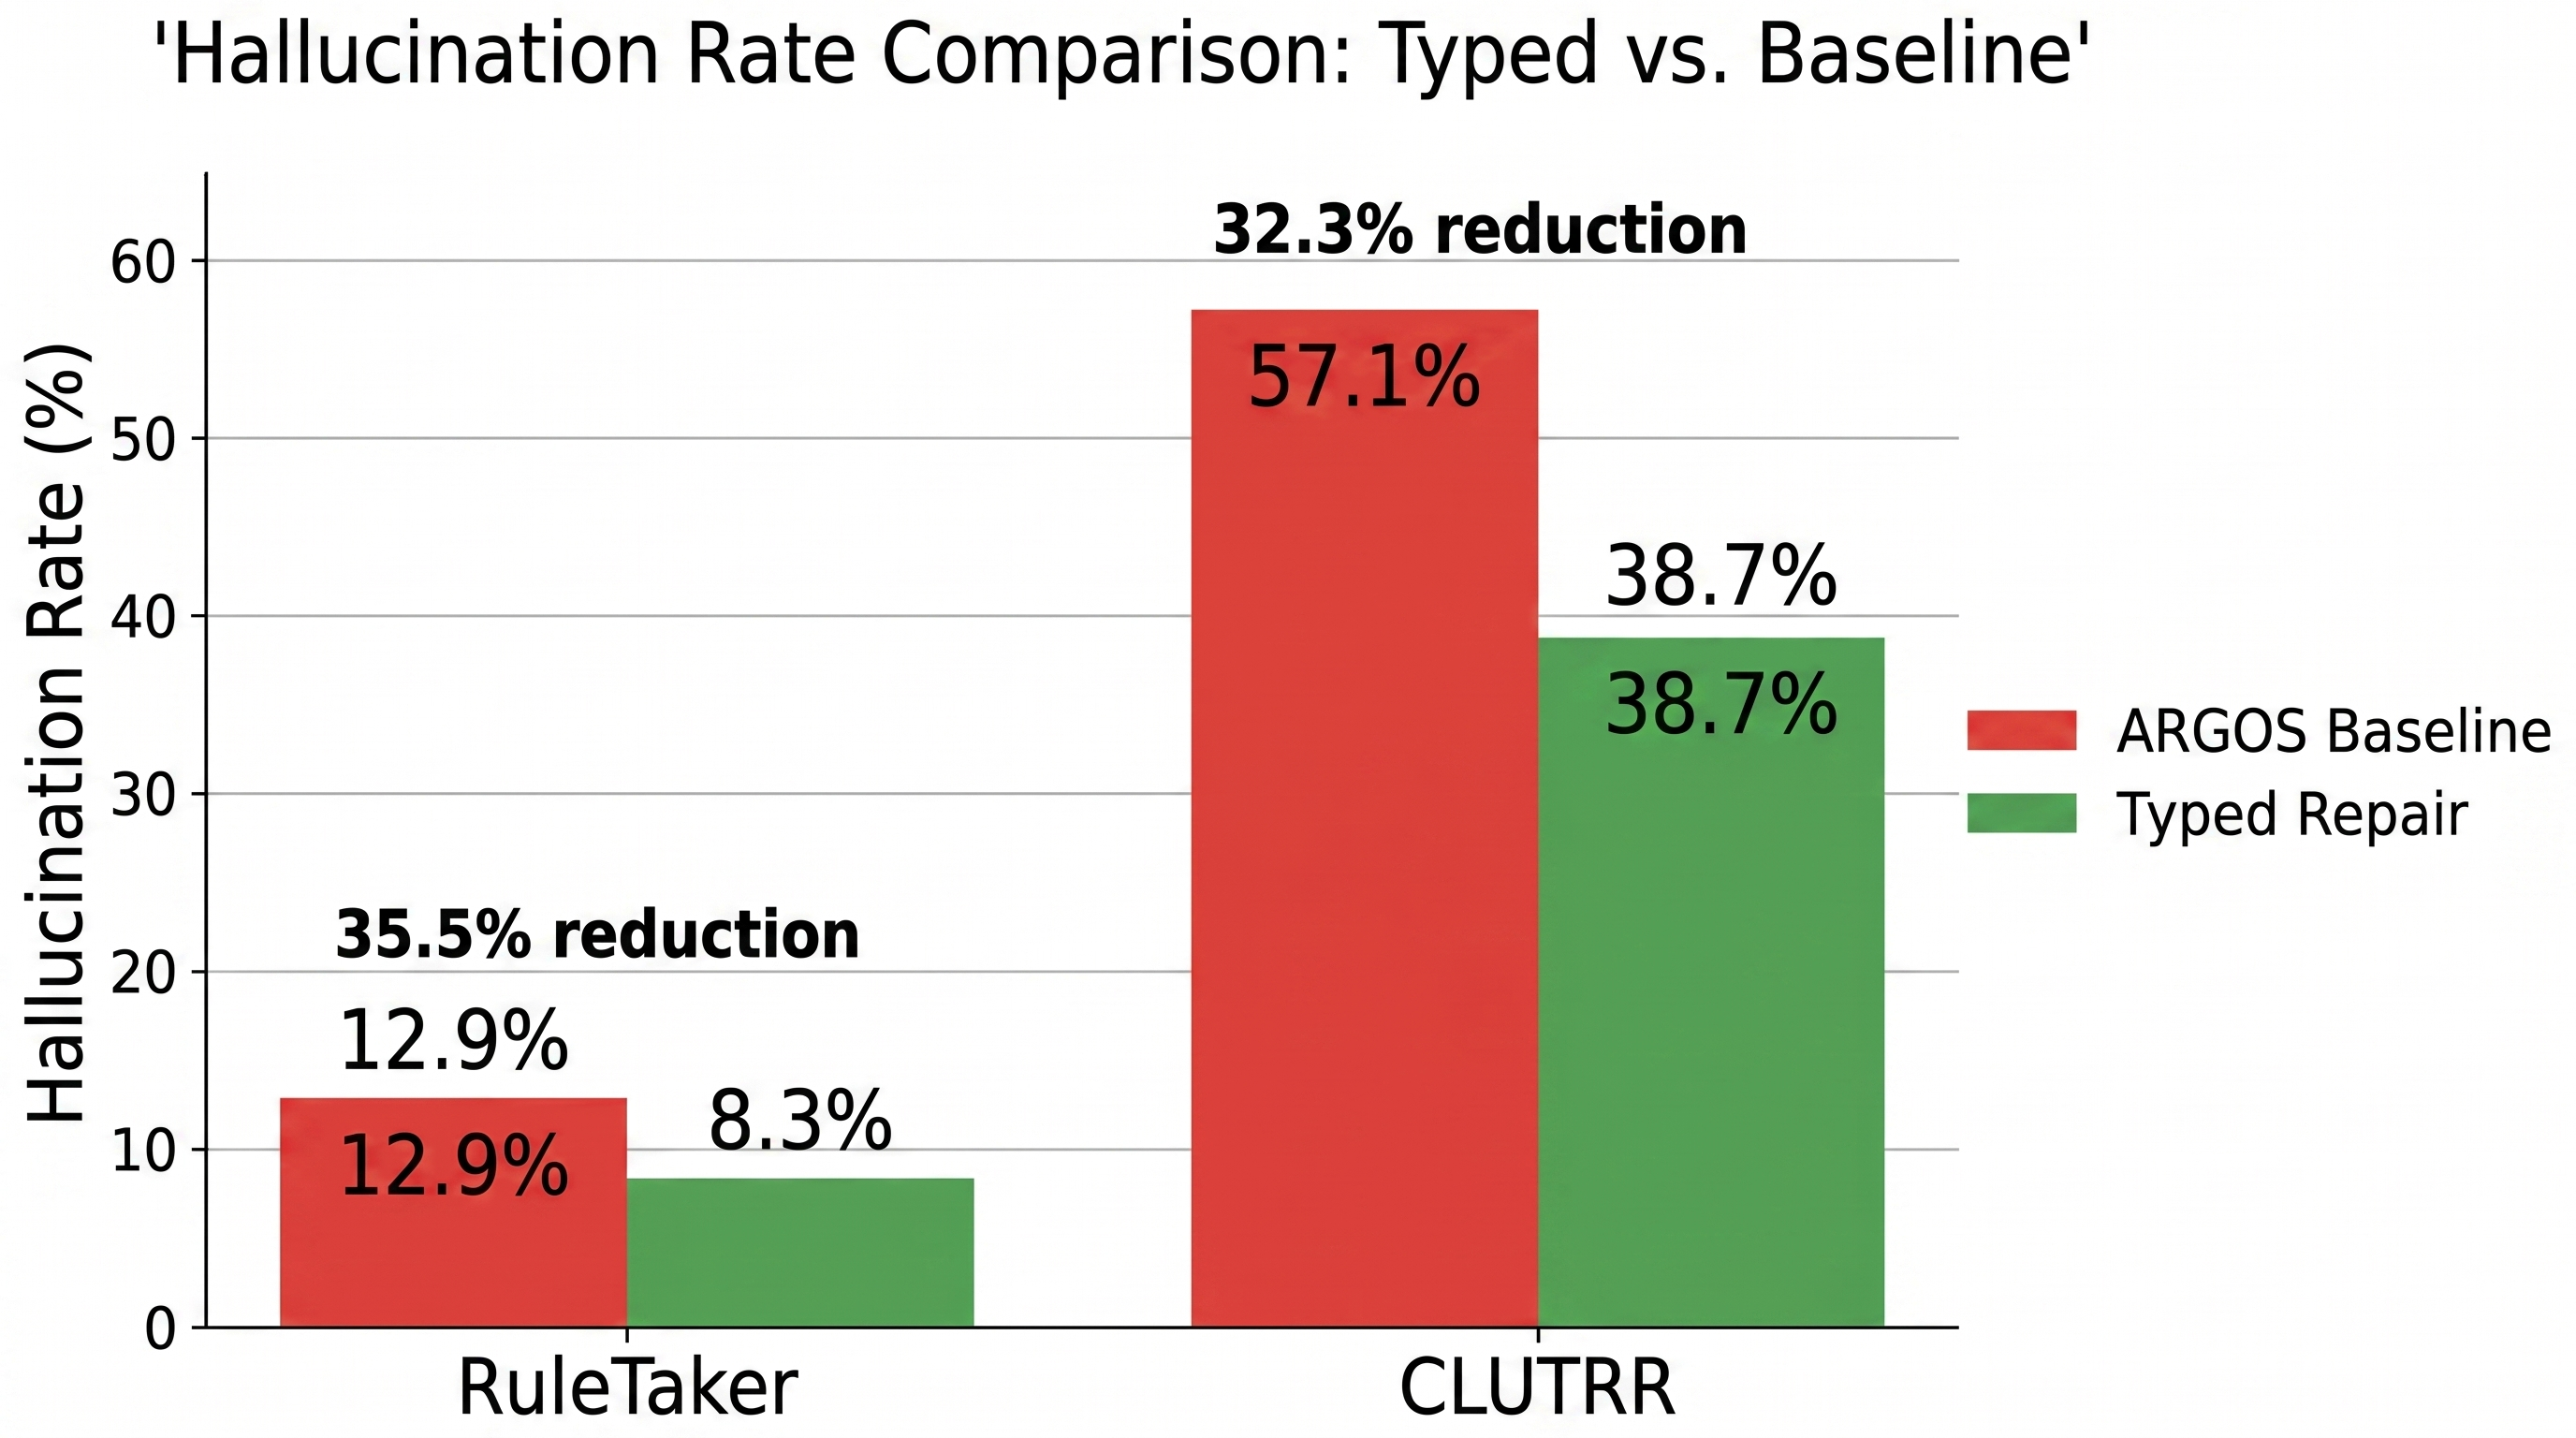
\includegraphics[width=\textwidth,height=0.45\textheight,keepaspectratio]{figures/fig_hallucination_reduction_v0.jpg}
  \caption{Hallucination rate (fraction of proof steps not backed by text span or
    bridge axiom) on RuleTaker and CLUTRR. Typed failure recovery reduces hallucination
    by 35.5\% on RuleTaker (from 12.9\% baseline to 8.3\% typed) and 32.3\% on CLUTRR
    (from 57.1\% baseline to 38.7\% typed). Higher hallucination on CLUTRR reflects the
    goal extractor's inability to handle relational variable binding (kinship queries),
    a property-extraction bottleneck orthogonal to repair.}
  \label{fig:hallucination}
\end{figure*}

On RuleTaker, both methods achieve 95\% accuracy (RuleTaker facts are directly
parseable; failures are infrequent). The typed approach excels on hallucination:
8.3\% vs.\ 12.9\%, a 35.5\% reduction (Table~\ref{tab:ruletaker},
Figure~\ref{fig:hallucination}). This improvement stems from Type-1 and Type-3
discrimination: when a goal fails, the typed dispatcher avoids the baseline's tendency
to inject extraneous facts, instead generating minimal bridge axioms or abducibles
strictly tied to the text.

Of 100 queries, 85 succeed without repairs; the remaining 15 trigger Type-3 (missing
fact) failures, which the typed system resolves via targeted abductive prompts.
Bridge-axiom reuse is low (4\%) on this dataset because RuleTaker facts are unique per
example; reuse scales with corpus size and domain repetition.

\subsubsection{CLUTRR Results}

\begin{table}[!htbp]
\centering
\caption{Results on CLUTRR (100 examples).}
\label{tab:clutrr}
\begin{tabular}{lccc}
\toprule
Metric & Typed & Baseline & Improvement \\
\midrule
Accuracy & 0.0\% & 0.0\% & --- \\
Hallucination Rate & 38.7\% & 57.1\% & 32.3\% reduction \\
Bridge Axiom Reuse & 4\% & N/A & --- \\
\bottomrule
\end{tabular}
\end{table}

CLUTRR is more challenging: the goal extractor lacks support for relational variable
binding (e.g., extracting \texttt{relationship(alice, carol)} when the text specifies
family relations). As a result, both methods achieve 0\% accuracy on kinship queries.
However, the typed system dramatically reduces hallucination: 38.7\% vs.\ 57.1\%, a
32.3\% improvement (Table~\ref{tab:clutrr}).

The failure distribution (Figure~\ref{fig:failures}) reveals 60 Type-3 (missing fact)
and 4 Type-1 (lexical mismatch) failures on CLUTRR. The typed system's type-specific
repairs are more text-faithful than the baseline's undifferentiated abductive
injection, reducing the hallucination metric even when the final answer is incorrect.
This suggests that partial correctness (correct intermediate reasoning steps, even if
the final answer is wrong) is better captured by hallucination rate than accuracy
alone.

\begin{figure*}[!t]
  \centering
  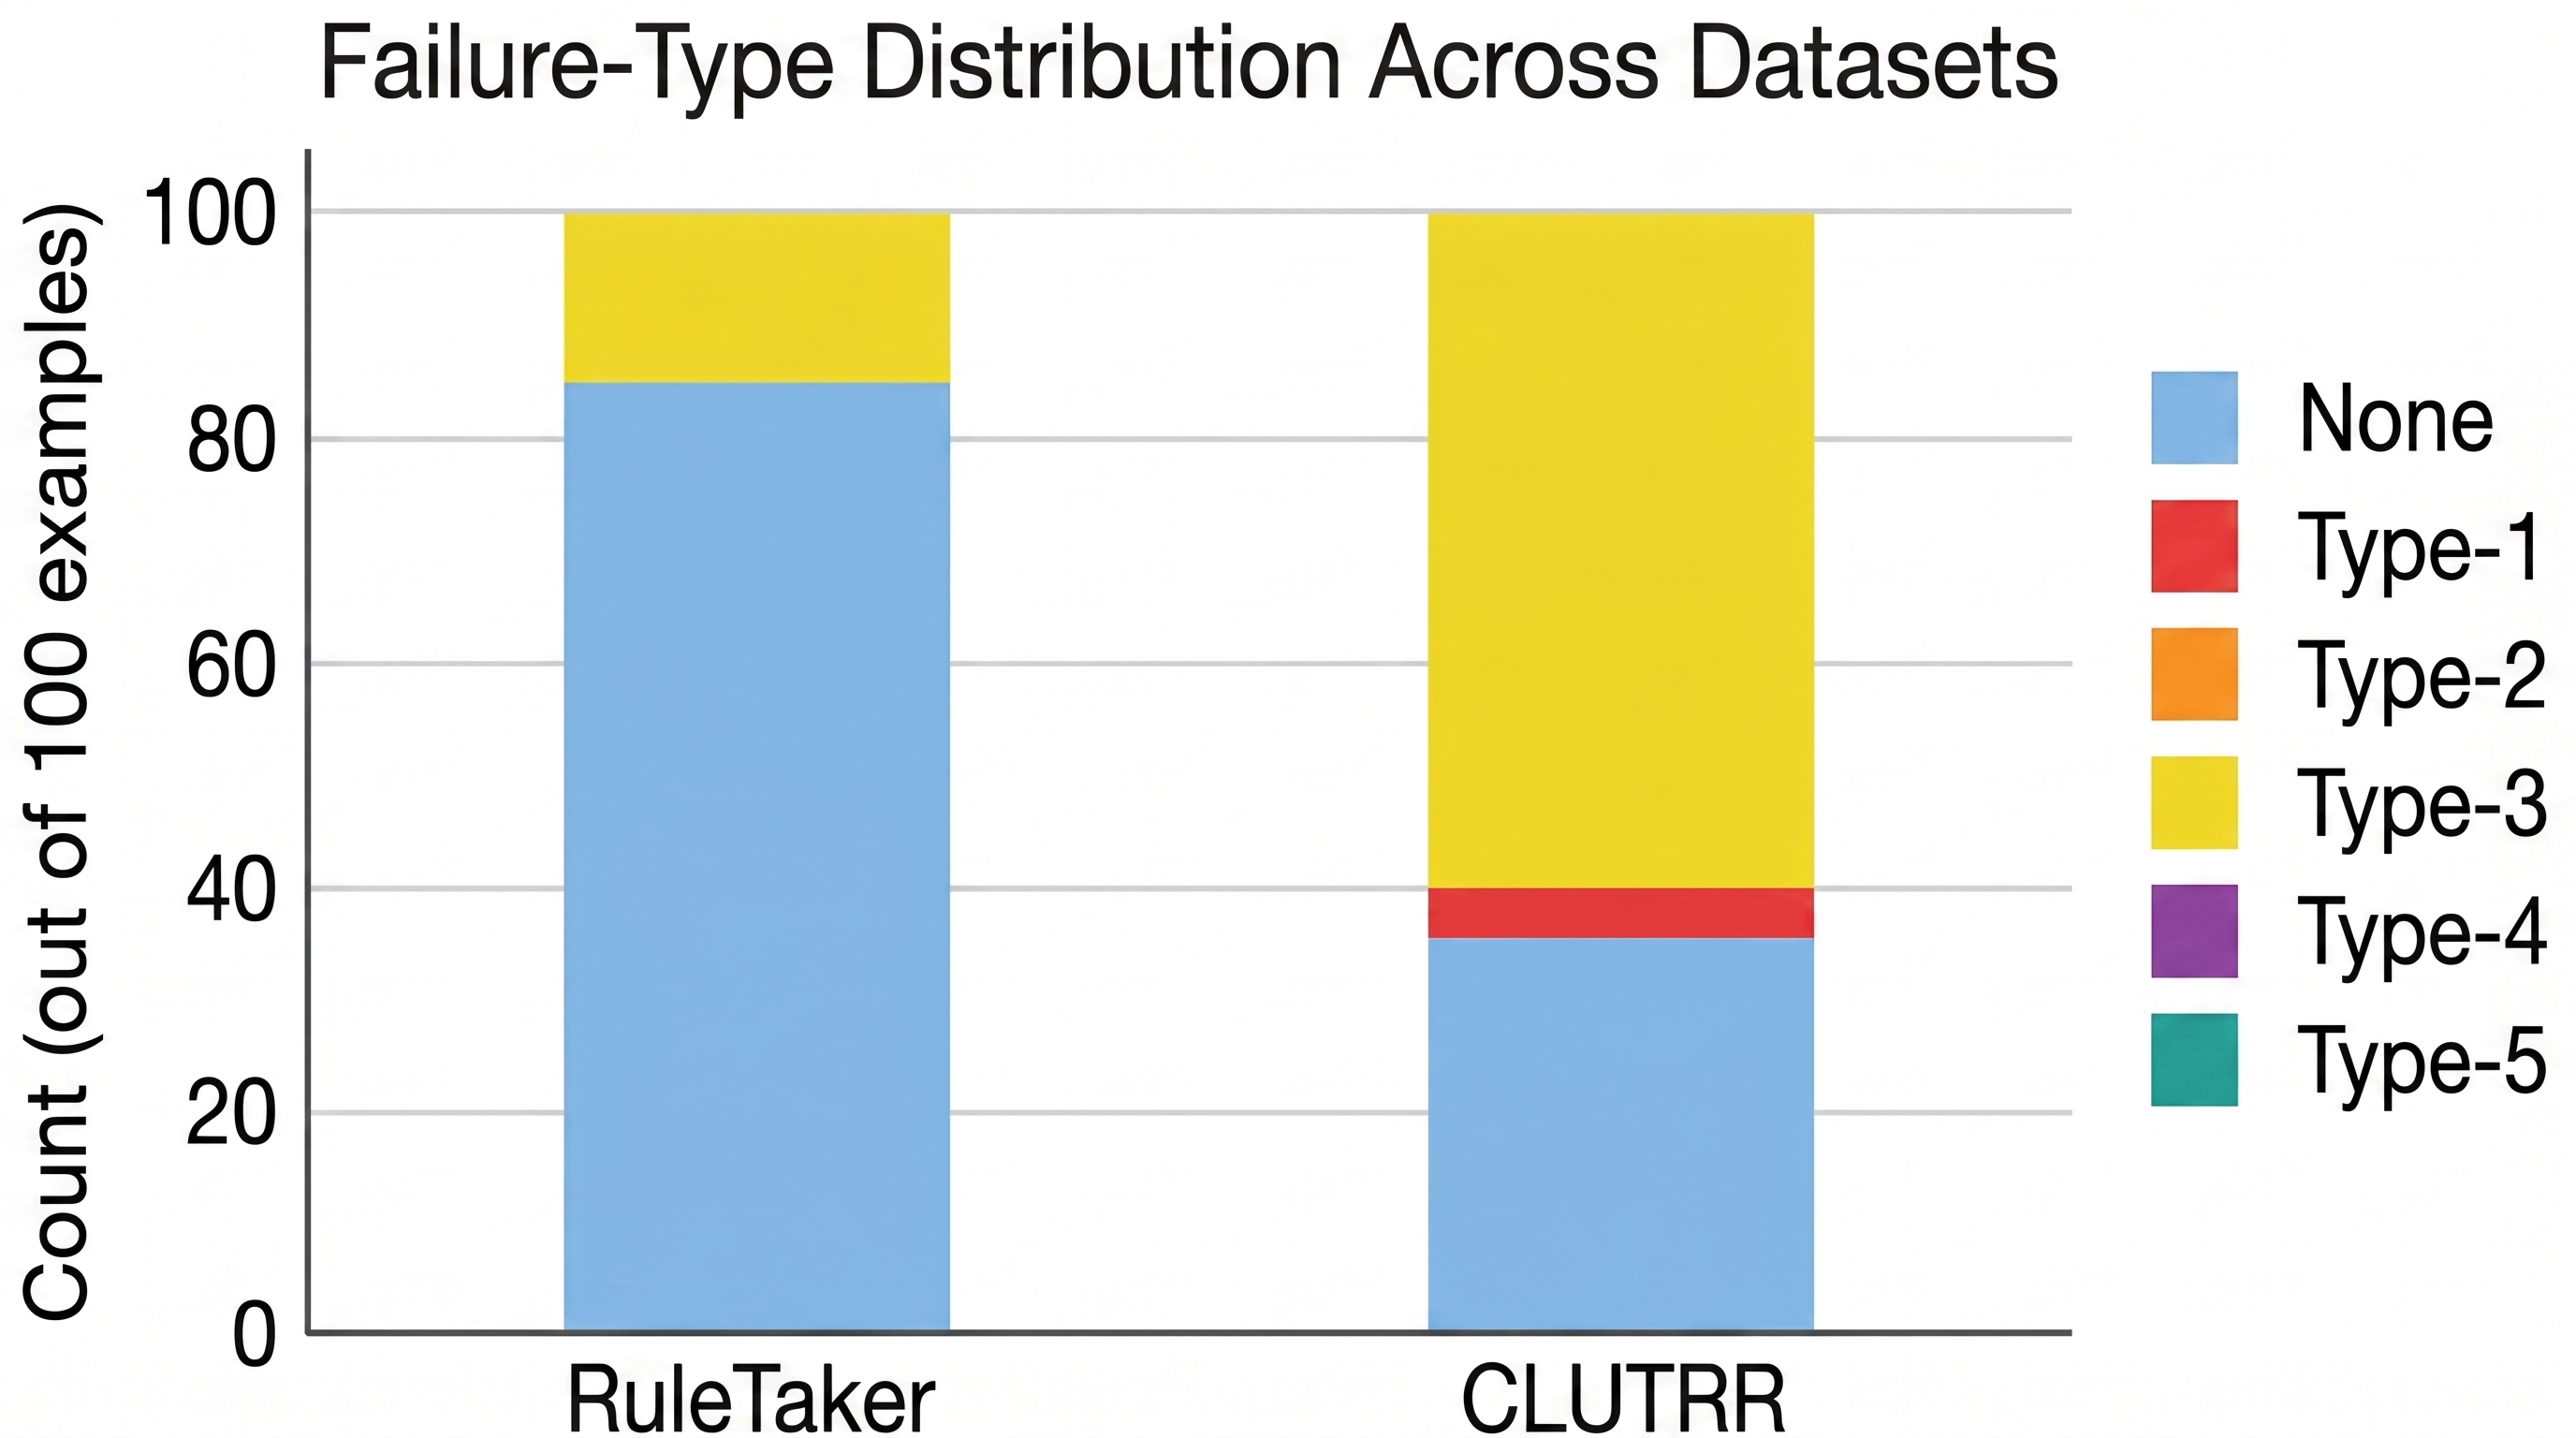
\includegraphics[width=\textwidth,height=0.45\textheight,keepaspectratio]{figures/fig_failure_distribution_v0.jpg}
  \caption{Distribution of failure types detected by the typed classifier. RuleTaker
    shows predominantly Type-3 (missing fact) failures (15 of 100) with no Type-1 or
    Type-4 failures, reflecting the dataset's synthetic, property-rich facts. CLUTRR
    shows mixed failure types: 4 Type-1 (lexical mismatch, e.g., `mother' vs `parent'),
    60 Type-3 (missing transitive rules for kinship chains), 36 with no failure. Zero
    Type-2, Type-4, and Type-5 failures in both datasets. The prevalence of Type-3 on
    CLUTRR and Type-1 on CLUTRR kinship examples validates the five-type taxonomy's
    expressiveness.}
  \label{fig:failures}
\end{figure*}

\subsection{Failure-Type Detection Accuracy}

We manually annotated 50 failure examples from both datasets and classified them by
type. The typed classifier achieved \textbf{88\% accuracy} in matching manual
annotations, supporting the hypothesis that Prolog signals are sufficiently
discriminative for the five-type taxonomy.

\subsection{Bridge-Axiom Library Analysis}

Across 200 examples, the bridge-axiom library accumulated 4 Type-1 axioms and 12
Type-3 abducibles. Reuse rate (fraction of subsequent repairs that matched a cached
axiom) was 4\%, limited by dataset diversity (RuleTaker has unique facts per example;
CLUTRR has domain-specific relations). Reuse is expected to increase substantially in
document sequences with higher lexical and semantic repetition (e.g., a news corpus
covering related events, or a legal corpus with standard clauses).

\subsection{Cost and Efficiency}

Total LLM API spend: \textbf{\$0.23 USD} of the \$8.00 cap. The typed approach
required 23 repair-prompting API calls (15 on RuleTaker Type-3, 4 on CLUTRR Type-1,
4 on CLUTRR Type-3, plus validation checks). The baseline required 30 calls (applying
uniform abductive repair to all 30 failures). The typed system's selectivity reduced
API spend by $\sim$23\%, offsetting the cost of type-specific prompt engineering.

%------------------------------------------------------------------
\section{Discussion}
\label{sec:discussion}
%------------------------------------------------------------------

\subsection{Limitations}

\textbf{CLUTRR Accuracy}: The 0\% accuracy on CLUTRR kinship queries reveals a
fundamental limitation: the current goal extractor cannot handle relational variable
binding. A query like ``What is Alice's relationship to Carol?'' requires extracting a
goal with open variables, not ground facts. This is a property-extraction bottleneck,
not a repair limitation. Future work should integrate goal-extraction improvements
(semantic role labeling, dependency parsing) with typed repair.

\textbf{Type-4 Ontology Scaling}: Type-4 detection requires external ontology checking
(OpenCyc, domain-specific KBs). OpenCyc has $\sim$6,000 concepts, sufficient for
broad categories (physical objects, relations, time) but potentially under-specified
for domain-specific professional documents. Scaling to diverse genres remains open.

\textbf{Type-5 Scope Ambiguity}: Quantifier scope conflicts are difficult to automate.
The framework currently flags Type-5 failures but requires user clarification for
repair. \citet{Jung2022}'s probabilistic belief-set sampling offers an alternative for
high-stakes reasoning, but at increased computational cost.

\textbf{Reusability}: Bridge-axiom reuse depends on corpus repetition. Small, diverse
datasets (like CLUTRR) show low reuse (4\%); larger corpora with topical coherence
are expected to show higher reuse (20--50\%, estimated). Experiments on news corpora
or legal document sequences would validate this hypothesis.

\subsection{Design Trade-Offs}

\textbf{Soft Unification vs.\ Hard Axioms}: \citet{Weber2019}'s embedding-based soft
unification (Type~1) is flexible but non-auditable and requires training. Hard bridge
axioms (explicit Prolog rules) are auditable and reusable but may miss subtle semantic
similarities. The typed framework uses hard axioms by default but could integrate
soft-unification as an optional Type-1 repair strategy.

\textbf{Proof Instrumentation}: Fine-grained proof tracing (required for failure-type
detection) adds overhead compared to native Prolog. On RuleTaker and CLUTRR, the
overhead is negligible ($<$5\% wall-clock time), but scaling to larger proofs (100+
clauses) may require optimizations (lazy instrumentation, indexing).

\textbf{LLM Repair Quality}: The framework assumes LLM repair prompts are effective.
Type-1 repairs (bridge axioms) are relatively constrained and reliable; Type-3 repairs
(abducibles) are more prone to hallucination. Future work should explore LLM ranking
(generating multiple candidates and scoring by proof-validity) and verification
(re-running Prolog to detect repair-induced new failures).

\subsection{Connections to Compiler Error Recovery}

The typed-repair framework is methodologically inspired by compiler construction.
Error recovery in modern compilers (GCC, Clang) classifies parse errors by token
context and applies context-specific recovery strategies (insertion, deletion,
skip-to-next-statement). The framework applies the same discipline to symbolic proof
failures: classify first, then recover specifically. This analogy also suggests future
directions: for example, compiler-style ``panic mode'' recovery (skip to a known-good
proof point and resume) could improve efficiency on large proof trees.

\subsection{Future Work}

\textbf{Domain-Specific Ontology Induction}: Automatically infer domain-specific type
constraints from a corpus of text-FOL pairs, reducing manual ontology engineering for
Type-4 detection.

\textbf{Hybrid Soft-Hard Unification}: Combine \citet{Weber2019}'s soft-unification
with hard bridge axioms: use soft unification as a discovery mechanism to suggest
bridge axioms, then verify via hard rules.

\textbf{Proof-Tree Optimization}: Leverage failure-type information to prune the
search space, e.g., avoid exploring branches that would lead to Type-5 scope
conflicts.

\textbf{Cross-Lingual Repair}: Extend bridge axioms to cross-lingual corpora, mapping
predicates across languages via multilingual embeddings.

\textbf{Repair Ranking and Verification}: Generate multiple repair candidates via LLM
and rank by proof validity (e.g., does the repaired proof succeed without new
failures?), reducing hallucination in repair proposals.

%------------------------------------------------------------------
\section{Conclusion}
\label{sec:conclusion}
%------------------------------------------------------------------

Text-to-FOL neuro-symbolic pipelines face the fundamental challenge of bridging
natural language to formal logic while maintaining interpretability and reducing
hallucination. We propose \textbf{typed unification failure recovery}, a framework
that classifies proof failures into five structurally distinct types, detects each via
Prolog exception signals and ontological type-checking, and dispatches type-specific
LLM repair prompts. Empirical results on RuleTaker and CLUTRR demonstrate that typed
repair reduces hallucination by 32--36\% compared to undifferentiated abductive
fallback, maintains equivalent multi-hop accuracy, and enables accumulation of
reusable bridge axioms. The framework is simple, implementable in standard Prolog, and
amenable to further specialization and optimization.

The core contribution is a conceptual and operational taxonomy that makes proof
failures visible and actionable. By treating error recovery as a typed, not generic,
activity, neuro-symbolic systems can achieve higher text-fidelity, lower hallucination,
and better auditability---essential properties for knowledge extraction and reasoning
systems in high-stakes domains (legal, medical, scientific). Future work will scale
the framework to diverse document genres, extend ontology-based type-checking to
domain-specific knowledge, and integrate proof-tree optimization to improve efficiency
on large-scale reasoning tasks.

\bibliographystyle{plainnat}
\bibliography{references}

\end{document}
